%================================================
%    sheaves on manifolds ノート
%================================================

% -----------------------
% preamble
% -----------------------
% ここから本文 (\begin{document}) までの
% ソースコードに変更を加えた場合は
% 編集者まで連絡してください. 
% Don't change preamble code yourself. 
% If you add something
% (usepackage, newtheorem, newcommand, renewcommand),
% please tell it 
% to the editor of institutional paper of RUMS.

% ------------------------
% documentclass
% ------------------------
\documentclass[11pt, a4paper, dvipdfmx, leqno]{jsarticle}

% ------------------------
% usepackage
% ------------------------
\usepackage{algorithm}
\usepackage{algorithmic}
\usepackage{amscd}
\usepackage{amsfonts}
\usepackage{amsmath}
\usepackage[psamsfonts]{amssymb}
\usepackage{amsthm}
\usepackage{ascmac}
\usepackage{bm}
\usepackage{color}
\usepackage{enumerate}
\usepackage{fancybox}
\usepackage[stable]{footmisc}
\usepackage{graphicx}
\usepackage{listings}
\usepackage{mathrsfs}
\usepackage{mathtools}
\usepackage{otf}
\usepackage{pifont}
\usepackage{proof}
\usepackage{subfigure}
\usepackage{tikz}
\usepackage{verbatim}
\usepackage[all]{xy}
\usepackage{url}
\usetikzlibrary{cd}



% ================================
% パッケージを追加する場合のスペース 
%\usepackage{calligra}
\usepackage[dvipdfmx]{hyperref}
\usepackage{xcolor}
\definecolor{darkgreen}{rgb}{0,0.45,0} 
\definecolor{darkred}{rgb}{0.75,0,0}
\definecolor{darkblue}{rgb}{0,0,0.6} 
\hypersetup{
    colorlinks=true,
    citecolor=darkgreen,
    linkcolor=darkred,
    urlcolor=darkblue,
}
\usepackage{pxjahyper}
\usepackage[mathscr]{euscript}
\usepackage{layout}
\usepackage{framed}
\definecolor{lightgray}{rgb}{0.75,0.75,0.75}
\renewenvironment{leftbar}{%
  \def\FrameCommand{\textcolor{lightgray}{\vrule width 0.7zw} \hspace{10pt}}% 
  \MakeFramed {\advance\hsize-\width \FrameRestore}}%
{\endMakeFramed}
\newenvironment{redleftbar}{%
  \def\FrameCommand{\textcolor{red}{\vrule width 1pt} \hspace{10pt}}% 
  \MakeFramed {\advance\hsize-\width \FrameRestore}}%
 {\endMakeFramed}

%=================================


% --------------------------
% theoremstyle
% --------------------------
\theoremstyle{definition}

% --------------------------
% newtheoem
% --------------------------

% 日本語で定理, 命題, 証明などを番号付きで用いるためのコマンドです. 
% If you want to use theorem environment in Japanece, 
% you can use these code. 
% Attention!
% All theorem enivironment numbers depend on 
% only section numbers.
\newtheorem{Axiom}{公理}[section]
\newtheorem{Definition}[Axiom]{定義}
\newtheorem{Theorem}[Axiom]{定理}
\newtheorem{Proposition}[Axiom]{命題}
\newtheorem{Lemma}[Axiom]{補題}
\newtheorem{Corollary}[Axiom]{系}
\newtheorem{Example}[Axiom]{例}
\newtheorem{Claim}[Axiom]{主張}
\newtheorem{Property}[Axiom]{性質}
\newtheorem{Attention}[Axiom]{注意}
\newtheorem{Question}[Axiom]{問}
\newtheorem{Problem}[Axiom]{問題}
\newtheorem{Consideration}[Axiom]{考察}
\newtheorem{Alert}[Axiom]{警告}
\newtheorem{Fact}[Axiom]{事実}
\newtheorem{com}[Axiom]{コメント}


% 日本語で定理, 命題, 証明などを番号なしで用いるためのコマンドです. 
% If you want to use theorem environment with no number in Japanese, You can use these code.
\newtheorem*{Axiom*}{公理}
\newtheorem*{Definition*}{定義}
\newtheorem*{Theorem*}{定理}
\newtheorem*{Proposition*}{命題}
\newtheorem*{Lemma*}{補題}
\newtheorem*{Example*}{例}
\newtheorem*{Corollary*}{系}
\newtheorem*{Claim*}{主張}
\newtheorem*{Property*}{性質}
\newtheorem*{Attention*}{注意}
\newtheorem*{Question*}{問}
\newtheorem*{Problem*}{問題}
\newtheorem*{Consideration*}{考察}
\newtheorem*{Alert*}{警告}
\newtheorem*{Fact*}{事実}
\newtheorem*{com*}{コメント}



% 英語で定理, 命題, 証明などを番号付きで用いるためのコマンドです. 
% If you want to use theorem environment in English, You can use these code.
%all theorem enivironment number depend on only section number.
\newtheorem{Axiom+}{Axiom}[section]
\newtheorem{Definition+}[Axiom+]{Definition}
\newtheorem{Theorem+}[Axiom+]{Theorem}
\newtheorem{Proposition+}[Axiom+]{Proposition}
\newtheorem{Lemma+}[Axiom+]{Lemma}
\newtheorem{Example+}[Axiom+]{Example}
\newtheorem{Corollary+}[Axiom+]{Corollary}
\newtheorem{Claim+}[Axiom+]{Claim}
\newtheorem{Property+}[Axiom+]{Property}
\newtheorem{Attention+}[Axiom+]{Attention}
\newtheorem{Question+}[Axiom+]{Question}
\newtheorem{Problem+}[Axiom+]{Problem}
\newtheorem{Consideration+}[Axiom+]{Consideration}
\newtheorem{Alert+}{Alert}
\newtheorem{Fact+}[Axiom+]{Fact}
\newtheorem{Remark+}[Axiom+]{Remark}

% ----------------------------
% commmand
% ----------------------------
% 執筆に便利なコマンド集です. 
% コマンドを追加する場合は下のスペースへ. 

% 集合の記号 (黒板文字)
\newcommand{\NN}{\mathbb{N}}
\newcommand{\ZZ}{\mathbb{Z}}
\newcommand{\QQ}{\mathbb{Q}}
\newcommand{\RR}{\mathbb{R}}
\newcommand{\CC}{\mathbb{C}}
\newcommand{\PP}{\mathbb{P}}
\newcommand{\KK}{\mathbb{K}}


% 集合の記号 (太文字)
\newcommand{\nn}{\mathbf{N}}
\newcommand{\zz}{\mathbf{Z}}
\newcommand{\qq}{\mathbf{Q}}
\newcommand{\rr}{\mathbf{R}}
\newcommand{\cc}{\mathbf{C}}
\newcommand{\pp}{\mathbf{P}}
\newcommand{\kk}{\mathbf{K}}

% 特殊な写像の記号
\newcommand{\ev}{\mathop{\mathrm{ev}}\nolimits} % 値写像
\newcommand{\pr}{\mathop{\mathrm{pr}}\nolimits} % 射影

% スクリプト体にするコマンド
%   例えば {\mcal C} のように用いる
\newcommand{\mcal}{\mathcal}

% 花文字にするコマンド 
%   例えば {\h C} のように用いる
\newcommand{\h}{\mathscr}

% ヒルベルト空間などの記号
\newcommand{\F}{\mcal{F}}
\newcommand{\X}{\mcal{X}}
\newcommand{\Y}{\mcal{Y}}
\newcommand{\Hil}{\mcal{H}}
\newcommand{\RKHS}{\Hil_{k}}
\newcommand{\Loss}{\mcal{L}_{D}}
\newcommand{\MLsp}{(\X, \Y, D, \Hil, \Loss)}

% 偏微分作用素の記号
\newcommand{\p}{\partial}

% 角カッコの記号 (内積は下にマクロがあります)
\newcommand{\lan}{\langle}
\newcommand{\ran}{\rangle}



% 圏の記号など
\newcommand{\Set}{{\bf Set}}
\newcommand{\Vect}{{\bf Vect}}
\newcommand{\FDVect}{{\bf FDVect}}
\newcommand{\Mod}{\mathop{\mathrm{Mod}}\nolimits}
\newcommand{\CGA}{{\bf CGA}}
\newcommand{\GVect}{{\bf GVect}}
\newcommand{\Lie}{{\bf Lie}}
\newcommand{\dLie}{{\bf Liec}}



% 射の集合など
\newcommand{\Map}{\mathop{\mathrm{Map}}\nolimits}
\newcommand{\Hom}{\mathop{\mathrm{Hom}}\nolimits}
\newcommand{\End}{\mathop{\mathrm{End}}\nolimits}
\newcommand{\Aut}{\mathop{\mathrm{Aut}}\nolimits}
\newcommand{\Mor}{\mathop{\mathrm{Mor}}\nolimits}

% その他便利なコマンド
\newcommand{\dip}{\displaystyle} % 本文中で数式モード
\newcommand{\e}{\varepsilon} % イプシロン
\newcommand{\dl}{\delta} % デルタ
\newcommand{\pphi}{\varphi} % ファイ
\newcommand{\ti}{\tilde} % チルダ
\newcommand{\pal}{\parallel} % 平行
\newcommand{\op}{{\rm op}} % 双対を取る記号
\newcommand{\lcm}{\mathop{\mathrm{lcm}}\nolimits} % 最小公倍数の記号
\newcommand{\Probsp}{(\Omega, \F, \P)} 
\newcommand{\argmax}{\mathop{\rm arg~max}\limits}
\newcommand{\argmin}{\mathop{\rm arg~min}\limits}





% ================================
% コマンドを追加する場合のスペース 
\renewcommand\proofname{\bf 証明} % 証明
\numberwithin{equation}{section}
\newcommand{\cTop}{\textsf{Top}}
%\newcommand{\cOpen}{\textsf{Open}}
\newcommand{\Op}{\mathop{\textsf{Open}}\nolimits}
\newcommand{\Ob}{\mathop{\textrm{Ob}}\nolimits}
\newcommand{\id}{\mathop{\mathrm{id}}\nolimits}
\newcommand{\pt}{\mathop{\mathrm{pt}}\nolimits}
\newcommand{\res}{\mathop{\rho}\nolimits}
\newcommand{\A}{\mcal{A}}
\newcommand{\B}{\mcal{B}}
\newcommand{\C}{\mcal{C}}
\newcommand{\D}{\mcal{D}}
\newcommand{\E}{\mcal{E}}
\newcommand{\G}{\mcal{G}}
%\newcommand{\H}{\mcal{H}}
\newcommand{\I}{\mcal{I}}
\newcommand{\J}{\mcal{J}}
\newcommand{\OO}{\mcal{O}}
\newcommand{\Ring}{\mathop{\textsf{Ring}}\nolimits}
\newcommand{\cAb}{\mathop{\textsf{Ab}}\nolimits}
\newcommand{\Ker}{\mathop{\mathrm{Ker}}\nolimits}
\newcommand{\im}{\mathop{\mathrm{Im}}\nolimits}
\newcommand{\Coker}{\mathop{\mathrm{Coker}}\nolimits}
\newcommand{\Coim}{\mathop{\mathrm{Coim}}\nolimits}
\newcommand{\Ht}{\mathop{\mathrm{Ht}}\nolimits}
\newcommand{\supp}{\mathop{\mathrm{supp}}\nolimits}
\newcommand{\colim}{\mathop{\mathrm{colim}}}
\newcommand{\Tor}{\mathop{\mathrm{Tor}}\nolimits}

\newcommand{\cat}{\mathscr{C}}

\newcommand{\scA}{\mathscr{A}}
\newcommand{\scB}{\mathscr{B}}
\newcommand{\scC}{\mathscr{C}}
\newcommand{\scD}{\mathscr{D}}
\newcommand{\scE}{\mathscr{E}}
\newcommand{\scF}{\mathscr{F}}

\newcommand{\ibA}{\mathop{\text{\textit{\textbf{A}}}}}
\newcommand{\ibB}{\mathop{\text{\textit{\textbf{B}}}}}
\newcommand{\ibC}{\mathop{\text{\textit{\textbf{C}}}}}
\newcommand{\ibD}{\mathop{\text{\textit{\textbf{D}}}}}
\newcommand{\ibE}{\mathop{\text{\textit{\textbf{E}}}}}
\newcommand{\ibF}{\mathop{\text{\textit{\textbf{F}}}}}
\newcommand{\ibG}{\mathop{\text{\textit{\textbf{G}}}}}
\newcommand{\ibH}{\mathop{\text{\textit{\textbf{H}}}}}
\newcommand{\ibI}{\mathop{\text{\textit{\textbf{I}}}}}
\newcommand{\ibJ}{\mathop{\text{\textit{\textbf{J}}}}}
\newcommand{\ibK}{\mathop{\text{\textit{\textbf{K}}}}}
\newcommand{\ibL}{\mathop{\text{\textit{\textbf{L}}}}}
\newcommand{\ibM}{\mathop{\text{\textit{\textbf{M}}}}}
\newcommand{\ibN}{\mathop{\text{\textit{\textbf{N}}}}}
\newcommand{\ibO}{\mathop{\text{\textit{\textbf{O}}}}}
\newcommand{\ibP}{\mathop{\text{\textit{\textbf{P}}}}}
\newcommand{\ibQ}{\mathop{\text{\textit{\textbf{Q}}}}}
\newcommand{\ibR}{\mathop{\text{\textit{\textbf{R}}}}}
\newcommand{\ibS}{\mathop{\text{\textit{\textbf{S}}}}}
\newcommand{\ibT}{\mathop{\text{\textit{\textbf{T}}}}}
\newcommand{\ibU}{\mathop{\text{\textit{\textbf{U}}}}}
\newcommand{\ibV}{\mathop{\text{\textit{\textbf{V}}}}}
\newcommand{\ibW}{\mathop{\text{\textit{\textbf{W}}}}}
\newcommand{\ibX}{\mathop{\text{\textit{\textbf{X}}}}}
\newcommand{\ibY}{\mathop{\text{\textit{\textbf{Y}}}}}
\newcommand{\ibZ}{\mathop{\text{\textit{\textbf{Z}}}}}

\newcommand{\ibx}{\mathop{\text{\textit{\textbf{x}}}}}

\newcommand{\Comp}{\mathop{\mathrm{C}}\nolimits}
\newcommand{\Komp}{\mathop{\mathrm{K}}\nolimits}
\newcommand{\Domp}{\mathop{\mathrm{D}}\nolimits}%複体のホモトピー圏

\newcommand{\CCat}{\Comp(\cat)}
\newcommand{\KCat}{\Komp(\cat)}
\newcommand{\DCat}{\Domp(\cat)}%圏Cの複体のホモトピー圏
\newcommand{\HOM}{\mathop{\mathscr{H}\hspace{-2pt}om}\nolimits}%内部Hom
\newcommand{\RHOM}{\mathop{\mathrm{R}\hspace{-1.5pt}\HOM}\nolimits}

\newcommand{\muS}{\mathop{\mathrm{SS}}\nolimits}
\newcommand{\RG}{\mathop{\mathrm{R}\hspace{-0pt}\Gamma}\nolimits}
\newcommand{\Rder}{\mathop{\mathrm{R}}\nolimits}

\newcommand{\simar}{\mathrel{\overset{\sim}{\longrightarrow}}}%内部Hom
\newcommand{\simra}{\mathrel{\overset{\sim}{\longleftarrow}}}%内部Hom

\newcommand{\hocolim}{{\mathrm{hocolim}}}
\newcommand{\indlim}[1][]{\mathop{\varinjlim}\limits_{#1}}
\newcommand{\sindlim}[1][]{\smash{\mathop{\varinjlim}\limits_{#1}}\,}
\newcommand{\Pro}{\mathrm{Pro}}
\newcommand{\Ind}{\mathrm{Ind}}
\newcommand{\prolim}[1][]{\mathop{\varprojlim}\limits_{#1}}
\newcommand{\sprolim}[1][]{\smash{\mathop{\varprojlim}\limits_{#1}}\,}

\newcommand{\Sh}{\mathrm{Sh}}
\newcommand{\PSh}{\mathrm{PSh}}


% =================================



%================================================
% 自前の定理環境
%   https://mathlandscape.com/latex-amsthm/
% を参考にした
\newtheoremstyle{mystyle}%   % スタイル名
    {5pt}%                   % 上部スペース
    {5pt}%                   % 下部スペース
    {}%              % 本文フォント
    {}%                  % 1行目のインデント量
    {\bfseries}%                      % 見出しフォント
    {.}%                     % 見出し後の句読点
    {12pt}%                     % 見出し後のスペース
    {\thmname{#1}\thmnumber{ #2}\thmnote{{\hspace{2pt}\normalfont (#3)}}}% % 見出しの書式

\theoremstyle{mystyle}
\newtheorem{AXM}{公理}[section]
\newtheorem{DFN}[Axiom]{定義}
\newtheorem{THM}[Axiom]{定理}
\newtheorem*{THM*}{定理}
\newtheorem{PRP}[Axiom]{命題}
\newtheorem{LMM}[Axiom]{補題}
\newtheorem{CRL}[Axiom]{系}
\newtheorem{EG}[Axiom]{例}
\newtheorem{CNV}[Axiom]{規約}
\newtheorem{CMT}[Axiom]{コメント}


% 定理環境ここまで
%====================================================

% ---------------------------
% new definition macro
% ---------------------------
% 便利なマクロ集です

% 内積のマクロ
%   例えば \inner<\pphi | \psi> のように用いる
\def\inner<#1>{\langle #1 \rangle}

% ================================
% マクロを追加する場合のスペース 

%=================================





% ----------------------------
% documenet 
% ----------------------------
% 以下, 本文の執筆スペースです. 
% Your main code must be written between 
% begin document and end document.
% ---------------------------

\title{超関数論文集}
\author{}
\date{}
\begin{document}
\maketitle
\section{関数概念の一般化について}

\subparagraph{1.}
L.シュヴァルツは\(C^\infty\)多様体上の関数概念を
\textbf{分布} (distribution) という概念の導入によって一般化した.
そしてこの概念は,解析学における様々な分野の間で,
広く用いることのできるものであることが明らかになった.\footnote{
    L.シュヴァルツ, 超関数の理論, Hermann (1950--1951).
}
ここでは,定義域の多様体が (\(C^\infty\)ではなく) 
\(C^\omega\)である場合に,関数概念の別の一般化の仕方を提案する.
ここでの一般化の仕方は,解析関数の境界値を用いるものである.
この新概念は\(C^\omega\)多様体の場合に,
シュワルツの分布を含む,より広い概念になっている.
この一般化 ``関数'' を\textbf{超関数} (hyperfunction) と
呼ぶことにする.正確には次のように定義する.
(議論を簡略化するため,ここでは1次元の場合の定義を述べるが,
\(C^\omega\)多様体上の超関数も定義できる.)\footnote{
    このノートの原稿を完成させた後,
    ``超関数''はG.ケーテ教授によって``Die...''において,
    すでに導入されていることを
    彌永教授を通じてA.ヴェイユ氏からご教示いただいた.
}




\begin{figure}[htb]
    \centering
    %\scalebox{0.8}{
        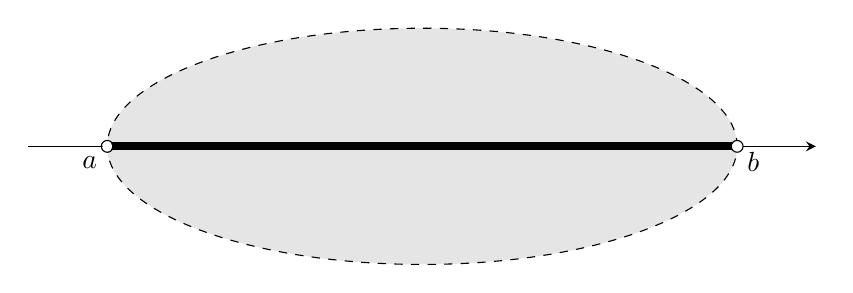
\begin{tikzpicture}[x=1cm]
        \fill[black!10] (0,0) ellipse (4 and 1.5);
        \draw[dashed,black!100] (0,0) ellipse (4 and 1.5);
        \draw[->,>=stealth,semithick] (-5,0)--(5,0)node[below]{$\RR$}; %x軸
        \draw[thick] (-4,0)--(4,0); %
        \fill[black!100] (-4,0.05) rectangle (4,-0.05);

        \draw[thick] (-4,-0.2) node[left]{\(a\)};
        \draw[thick] (4,-0.2) node[right]{\(b\)};
        %\draw (-1.3,0.1) node[above]{$F$};
        \draw (1.3,-1) node[left]{$\varOmega$};

        \fill[black!0](4,0) ellipse (0.075 and 0.075);
        \draw (4,0) ellipse (0.075 and 0.075);

        \fill[black!0](-4,0) ellipse (0.06 and 0.075);
        \draw (-4,0) ellipse (0.075 and 0.075);
    \end{tikzpicture}%}
    \caption{超関数のアレ}
    \label{fig:cpx-neiborhood}
\end{figure}







%===============================================
% 参考文献スペース
%===============================================
\begin{thebibliography}{20} 
    \bibitem[B+84]{B+84} Borel, 
        \textit{Intersection Cohomology}, 
        Progress in Mathematics, 50, Birkh\"auser, 1984.
    \bibitem[KS90]{KS90} Masaki Kashiwara, Pierre Schapira, 
        \textit{Sheaves on Manifolds}, 
        Grundlehren der Mathematischen Wissenschaften, 292, Springer, 1990.
    \bibitem[KS06]{KS06} Masaki Kashiwara, Pierre Schapira, 
        \textit{Categories and Sheaves}, 
        Grundlehren der Mathematischen Wissenschaften, 332, Springer, 2006.
    \bibitem[Sh16]{Sh16} 志甫淳, 層とホモロジー代数, 共立出版, 2016.
    \bibitem[Ike21]{Ike21} 池祐一, 超局所層理論概説, 2021.
    \bibitem[Tak17]{Tak17} 竹内潔, \(\D\)加群, 共立出版, 2017.
    %\bibitem[Og02]{Og02} 小木曽啓示, 代数曲線論, 朝倉書店, 2022.
\end{thebibliography}

%===============================================


\end{document}
